
\thispagestyle{empty}

\chapter{Visual stability across combined eye and body motion}
\chaptermark{}


\newpage

\small {\bf Abstract} In order to maintain visual stability during self-motion, the brain needs to update any ego-centric spatial representations of the environment. Here, we use a novel psychophysical approach to investigate how, and to which extent, the brain integrates visual, extraocular, and vestibular signals pertaining to this spatial update. Participants were oscillated sideways at a frequency of 0.63 Hz while keeping gaze fixed on a stationary light. When the motion direction changed, a reference target was shown either in front or behind the fixation point. At the next reversal, half a cycle later, we tested updating of this reference location by asking participants to judge whether a briefly flashed probe was shown to the left or right of the memorized target. We show that updating is not only biased, but that the direction and magnitude of this bias depend on both gaze and object location, implying that a gaze-centered reference frame is involved. Using geometric modeling, we further show that the gaze-dependent errors can be caused by an underestimation of translation amplitude, by a bias of visually perceived objects towards the fovea (i.e., a foveal bias), or by a combination of both.

\vfill

\noindent\underline{ \hspace{4cm} }

\noindent This chapter has been published as \newline
\noindent {\bf Clemens, I.A.H.}, Selen, L.P.J., Koppen, M. and Medendorp, W.P. \citeyear{clemens2012}. Visual stability across combined eye and body motion. \emph{Journal of Vision}, 12(12):8 1-11. \newline

\newpage


\section{Introduction}

A typical characteristic of human vision is that the position of the retina is constantly changing due to eye, head, and/or body movements. Yet, even during such self-motion, we retain a sense of whether visual objects are stable or moving with respect to an earth-centric reference frame (see e.g. Wallach, 1987). This capability is essential for a correct percept of the world and the maintenance of visual stability. 
Achieving visual stability is a complex process because visual signals are coded with respect to gaze, and not in an earth-fixed reference frame. When the visual scene lacks earth-centric landmarks, the brain should distinguish which changes in retinal input result from real world movement and which from eye movement. The usual view, dating back to Von Helmholtz (1867), is that this is achieved by subtracting the extraretinal signal of eye motion from the retinal image shifts \cite{wexler2005}.
Visual stability experiments in which participants made head-fixed saccades suggest that efference copies of the outgoing motor commands serve this purpose. Neurons in the frontal eye fields and the lateral intraparietal area demonstrate pre-saccadic shifts of receptive fields, elicited by an efference copy \cite{duhamel1992, kusunoki2003}. These gaze-centered shifts could allow the brain to anticipate and cancel out the changes in retinal input due to the saccade \cite{sommer2006}. Also, fMRI studies have reported evidence for shifting receptive fields in the human brain \cite{medendorp2003a}. 
Despite these important insights, head-fixed saccades are only one of a multitude of movements that are made in real life. Bringing the body in motion, like when driving a car, puts severe challenges on the mechanism underlying visual stability. In this case, when the body is translated passively, vestibular feedback informs the brain about the motion. This information must be combined with efference copies of orbital eye movements to interpret the changes in retinal input. Solving this problem is geometrically complicated because, during eye and body motion, the changes in retinal input depend nonlinearly on the depth and direction of objects that make up the retinal image, as in motion parallax \cite{medendorp2003b}.
Recent studies have reported fairly accurate reach or gaze responses to memorized target locations, presented prior to whole-body translations (see for review: Klier and Angelaki, 2008; Medendorp, 2011). However, such studies do not map one-to-one to the mechanisms of visual stability. First, the requirement of a motor response may invoke different processing mechanisms, which may be subject to different constraints. Second, motor response studies probe the system after the limb or eye movement, thereby revealing the combined result of all intervening spatial computations and transformations needed to guide the action. 
In the present study, we investigate visual stability across simultaneous eye and whole-body motion without involving the motor system. To this end, we used a two-alternative forced choice (2-AFC) psychophysical approach in combination with a visual updating paradigm. Participants had to retain object locations during sinusoidal whole-body motion, while keeping their gaze fixed on a world stationary point either in front of or behind the object.
By systematically manipulating the parameters of retinal and extraretinal signals related to body translation, binocular fixation, and object location, we test how the brain integrates these signals for the maintenance of visual stability. Our results show consistent errors in visual stability, which strongly depend on the location of the object relative to gaze. Using a modeling approach, we explore possible causes underlying these gaze-centered updating errors.


\section{Methods}

\subsection{Participants}

Eight participants (4 male, 4 female), aged between 22 and 41 years, provided written informed consent to participate in the experiment. All participants were free of any known vestibular or neurological disorder and had normal or corrected-to-normal visual acuity. Three participants (the authors) were knowledgeable about the purpose of the experiment, but their results did not differ from the five na�ve subjects. Participants never received any feedback about their performance.

\subsection{Setup}

A linear sled on a 800mm track was used to laterally translate participants. The sled, powered by a linear motor (TB15N, Technotion, Almelo, The Netherlands), was controlled by a Kollmorgen S700 (Danaher, Washington DC, USA) drive. The kinematics of the sled were controlled with an accuracy better than 34 ?m, 2 mm/s, and 150 mm/s2. The sled was configured such that participants were seated on the sled with the interaural axis aligned with the motion axis. Participants were restrained using a 5-point seat belt and a chin rest. In addition, the head was firmly held in place using an ear-fixed mold.  Emergency buttons at both sides of the sled chair enabled subjects to stop the sled motion immediately if needed. Eye movements were recorded using an EyeLink II (SR Research, Kanata, Canada) eye tracking system. Its camera system, which was mounted to the sled, remained stable with respect to the head during the entire experiment. Eye positions were calibrated based on the visual fixations during the experiment, under the assumption that these fixations were accurate.

\subsection{Visual stimuli}

Participants had to memorize the location of a earth-centric visual target (reference, R) during half a period of sinusoidal body translation. We tested the quality of this memory by asking them to judge and report the position of a probe stimulus (P) relative to that memorized location, following a psychophysical procedure. The reference and probe stimuli were both presented using a one-dimensional 450mm wide array, consisting of 180 red light emitting diodes (LEDs), with a spatial separation of 2.5 mm between neighboring LEDs. The LED array was oriented in parallel with the motion direction of the sled, centered w.r.t. the sled's trajectory and at the same vertical level as the participant's eyes. It was positioned with an accuracy better than 5 mm, at one of five different distances (850, 1050, 1200, 1400, or 2070 mm) from the participant's eyes in front of the sled. We further positioned an LED at either 850, 1050, 1200, 1400, or 2070 mm in front of the participant, on a virtual line orthogonal to the sled's motion direction and crossing the center of the LED array. These latter LEDs served as earth-stationary gaze fixation points (FP) during the experiment, so that gaze was directed either behind or in front of the stimulus array. The fixation points were displaced vertically by a few mm, such that the fixation point and the LED array did not occlude each other.

\subsection{Paradigm}

The experiments employed a paradigm that studies the constancy of spatial locations during 0.63 Hz sinusoidal whole-body motion in the lateral direction (left-right motion). We tested the effects of body translation (T, 150 or 300 mm peak-to-peak amplitude), fixation depth (FP, four spatial locations), and depth of the reference target (R, four spatial locations) on the quality of perceptual stability. These quantitative data will be interpreted using the geometric framework outlined in the subsection Model below.

\begin{figure}
	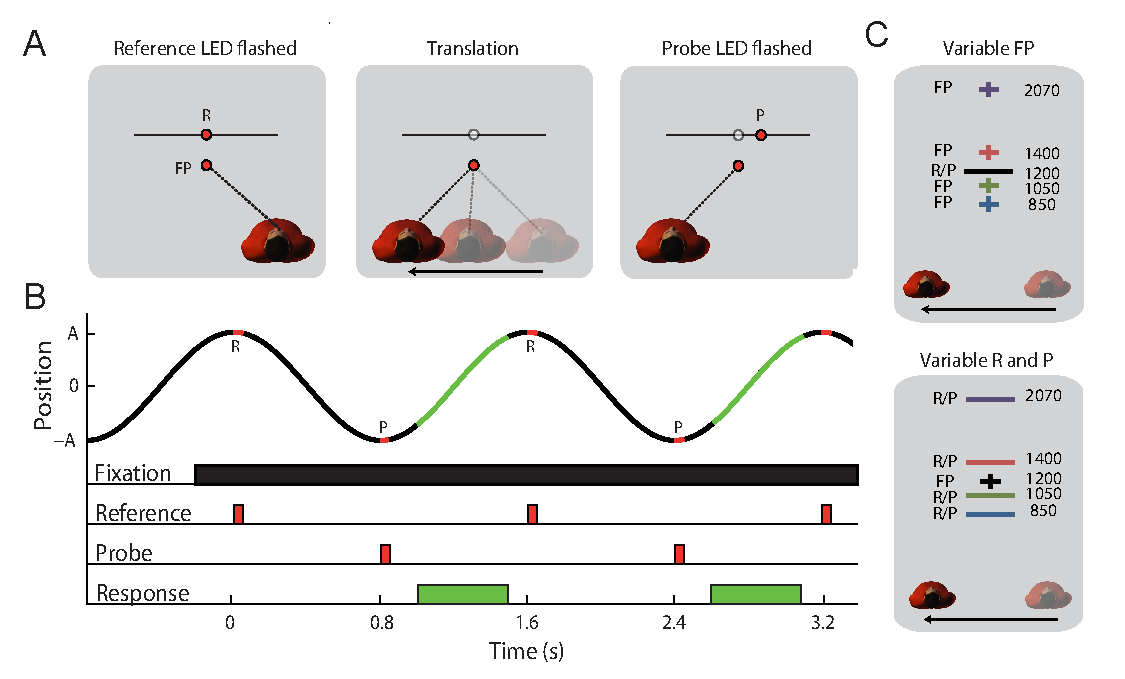
\includegraphics[width=1.0\textwidth]{src/paper2/figure1.pdf}
\end{figure}

Figure 1, panels A and B, illustrate the paradigm in detail; Figure 1C provides an overview of the experimental conditions. The experiment consisted of runs of either 30 or 15 trials. Each run started with the onset of a FP, to be fixated for the entire duration of the run. To avoid discontinuous acceleration at motion onset, sled velocity was linearly increased over one sinusoidal cycle (see Merfeld, Park, Gianna-Poulin, Black, and Wood, 2005 for a similar approach). Once the steady-state sinusoidal motion was reached, participants were tested using a visual updating task (Figure 1A). More specifically, at the most rightward position, when the body motion reversed direction, the reference R (here, the center LED) was presented for 50 ms. When the sled reached the left-most position, again during motion reversal, the participant's estimate for the location of R was tested by displaying another LED, the probe P, for 50 ms. The participant then had to report the location of this probe relative to R in a two-alternative forced choice (leftward, rightward) using a joystick. While we asked participants to respond in a timely manner, we did not explicitly constrain response time. Therefore, the next trial was only presented after a response was given. In practice, most responses were given within half a cycle (RT �SD = 0.59s �0.09, across participants). We used an adaptive algorithm to vary the spatial separation between reference and probe target from trial to trial \cite{kontsevich1999}, mapping out psychometrically the bias and precision of visual stability across whole-body motion. 
Participants were tested in 16 conditions, each comprising a unique combination of translation amplitude (T), visual fixation point (FP), and reference (R) position (see Fig 1C). The values used in this experiment are shown in Table 1. For each condition we presented 135 trials, which were divided into 4 runs of 30 trials and one run of 15 trials. In every condition 70 out of 135 trials were normal trials, that is, the central LED was used as reference. The other 65 trials in each condition were catch trials, of which 25 trials had the reference location shifted 36 mm to the left of the central led; another 25 had the reference location 36 mm rightward, and in 15 trials a random LED in the stimulus array was taken as the reference location. The catch trials were to prevent participants from simply making repeated stereotypic responses. After each run, the lights were turned on. Following a 30 s break, the experiment resumed automatically. The total experiment was divided into three sessions, tested on different days.  Each participant was tested on a total of 2160 trials.

% Table 1

\subsection{Data analysis}

To prevent effects caused by vergence and/or version eye-movements, we excluded trials in which participants did not maintain fixation within a 3 degree interval around FP, during the time interval starting 100ms before presenting the reference target and ending 100ms after cueing the probe. Overall, 6.4\% �1.7\% ({\textpm}SD) of all trials were discarded per participant based on these eye movement criteria. 
For each condition, we quantified performance by calculating the probability of a rightward response as a function of the location of the probe relative to reference location. We used a maximum likelihood fit of a cumulative Gaussian function to summarize the psychometric data:

\begin{equation}
\label{p1psych}
P(x) = \lambda + (1 - 2\lambda) \frac{1}{\sigma \sqrt{2\pi}} \int_{-\infty}^{x}{e^{-(y-\mu)^2 / 2\sigma^2}}dy,
\end{equation}

in which x represents the size of probe displacement. The mean of the Gaussian, $\mu$, represents the bias in visual stability (positive $\mu$ corresponding to a rightward bias). The width of the curve, corresponding to the standard deviation $\sigma$ of the Gaussian, is inversely related to precision, and serves as a measure of the participant's variability in the visual updating task. Parameter $\lambda$, representing the lapse rate, accounts for stimulus-independent errors caused by subject lapses or mistakes and was restricted to small values ($\lambda < 0.06$). Fits were performed using the 'psignifit' Matlab toolbox \cite{wichmann2001, wichmann2001b}.


\subsection{Model}

We investigated whether the observed bias can be explained by allowing a gain factor in the processing of the lateral translation by the vestibular system. That is, we assume that $\tilde{T} = {\alpha}T$, where $\tilde{T}$ is the perceived and $T$ the actual translation (Medendorp, Van Asselt, and Gielen, 1999). If the spatial update is performed entirely in a head-centered system, the effect of this gain would be straightforward. The reference flash $R$ is presented when the sled is in the rightmost position and the following translation of the sled by $T$ mm to the left in world coordinates amounts to a translation of the world, including the reference point, by $T$ mm to the right in head-coordinates. Due to the gain of the vestibular system the perceived translation equals ${\alpha}T$ mm to the right, leading to a predicted bias of

\begin{equation}
\mu = \tilde{T} - T = (\alpha - 1) T
\end{equation}

in mm on the LED array. Thus, when processed in a head-centered system, the bias would be negative for $\alpha < 1$, positive for $\alpha > 1$; it would be proportional to the translation amplitude, but would not depend at all on the reference and fixation point positions.
Previous experiments \cite{vanpelt2007} have shown that reach targets are updated not in head-centered coordinates, but rather within a gaze-dependent frame of reference. Following up on this, we also model the effect of the translation gain in a gaze-centered system. Let OF be the vector from the cyclopean eye to the fixation point and, similarly, $OR$ the vector to the reference point. The translation by $T$ mm to the left in world coordinates is in head-coordinates well approximated by a rotation of OF by $T/|OF|$ radians to the right and a rotation of OR by $T/|OR|$ radians to the right. (The approximation is good, since both $T<<|OF|$ and $T<<|OR|$. To express the gist of the prediction of the gaze-dependent model, this first-order approximation is very useful; in the actual calculations the precise geometry was used, without noticeable differences.)  Consequently, in gaze-centered coordinates (i.e., OF fixed straight ahead) the vector OR rotates by an angle of 

\begin{equation}
\phi \approx T (\frac{1}{|OR|} - \frac{1}{|OF|})
\end{equation}

radians to the right. In modeling the perceived rotation angle $\tilde{\phi}$ we again replace $T$ by $\tilde{T} = {\alpha}T$, but we also have to consider possible biases in the perception of $|OR|$ and $|OF|$. Following previous literature \cite{gogel1977, medendorp2003b}, we assume that the depth of the constantly visible fixation point is perceived accurately, i.e., $|\tilde{OF}| = |OF|$, but we allow that the perceived depth of the 50 ms flashed reference stimulus, $|\tilde{OR}|$, is biased towards this fixation point depth. Since the depth signals available in this experiment (vergence angle and disparity) express more directly in terms of inverse depth than depth itself. The simplest way to implement such a bias is to model the perceived reference depth as a weighted harmonic mean of the actual reference and fixation depths:

\begin{equation}
\frac{1}{|\tilde{OR}|} = \beta \frac{1}{|OR|} + (1 - \beta) \frac{1}{|OF|}
\end{equation}

where $\beta = 1$ represents the limiting case of accurate depth perception of the reference stimulus (no bias) and $\beta = 0$ the limiting case of full "assimilation" to fixation point depth. In total this leads to a perceived rotation angle of

\begin{equation}
\tilde{\phi} = {\alpha}T \cdot \beta(\frac{1}{|OR|} - \frac{1}{|OF|})
\end{equation}

radians to the right. Comparing Eq. 5 with Eq. 3 shows that our assumptions amount to a total gain of $\alpha\beta$ on the rotation angle, with freely interchangeable contributions of the parameters $\alpha$ and $\beta$. We substitute $\gamma = \alpha\beta$ and note that the resulting bias in angle, $\tilde{\phi} - \phi$, is observed as a bias in mm on the LED array at a distance $|OR|$:

\begin{equation}
\mu = (\tilde{\phi} - \phi)|OR| = (\gamma - 1)T(1 - \frac{|OR|}{|OF|})
\end{equation}

Thus, in the gaze-centered model the bias is again proportional to translation amplitude, but now it also depends critically on the fixation and reference point positions. In particular, the bias flips sign according to presenting the reference point in front of or behind the fixation point. On top of this, there is an overall (across all conditions) sign dependence on the combined values of the translation gain and fixation depth bias factors.

\section{Results}

Participants were tested in an experimental paradigm that studies the stability of spatial locations across combined eye and body motion. The task, illustrated in Figure 1, requires that subjects fixate an earth-stationary central fixation point, FP, which is visible throughout the run. At two successive reversals of motion direction, at the right and left excursion point of the sinusoidal motion, a reference (R) and a probe (P) target are briefly flashed. In a two-alternative forced choice task, the participant has to indicate whether the probe location was to the left or to the right of the reference location. The resulting psychometric data provide a quantitative assessment of the bias ($\mu$) and precision ($\sigma^{-2}$) of visual stability across self-motion (see Methods for details). Depending on the stimulus conditions (FP, R, and T), participants may erroneously judge the location of R, and hence provide biased responses.

Figure 2 shows the results of a typical participant, plotting the fraction of rightward responses (indicated by the circles) as a function of horizontal probe location relative to the reference. The 16 conditions are split into 4 panels according to the manipulated variable: FP distance (top panels), reference distance (bottom panels) and translation amplitude (left vs. right panels). Data for all individual probes are presented (circles). In an ideal observer, all psychometric functions would constitute a step response centered at zero, indicating no bias and no uncertainty. However, the actual data show consistent biases and non-zero variance.
When FP was behind R, we observed a leftward bias (top panels; red and purple curves), that increased when fixation was further away from the reference location (red vs. purple dots). When FP was in front of R (green and blue dots), the opposite pattern was seen. Furthermore, as T increases, psychometric curves move away from zero (t-test; $t(63) = -4.55$, $p < 0.05$) and become less steep (t-test; $t(63) = -4.64$, $p < 0.05$), a sign that there is decay in both accuracy and precision (compare left and right panels). Similar biases are observed when keeping FP constant, and varying the location of R, as demonstrated by the bottom panels. We derived estimates of the bias ($\mu$) and corresponding standard deviation ($\sigma$) values in each of the 16 conditions, for all subjects.

\begin{figure}
    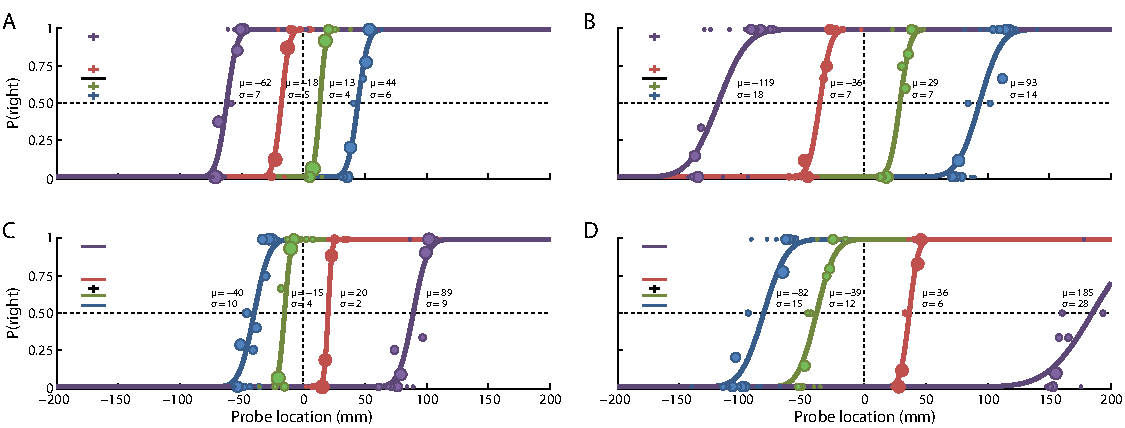
\includegraphics[width=1.0\textwidth]{src/paper2/figure2.pdf}
\end{figure}

Figure 3 depicts the bias ($\mu$) for each subject (dots), together with the mean bias {\textpm}SD across subjects (error bars), in top-view panels. This shows that the pattern in Figure 2 holds across all participants, with biases ranging between -126 and 212 mm. Clearly, the bias in updating of the central target increases with T and depends on FP, reversing for gaze fixation behind versus in front of the R (two top panels). Likewise, when FP was kept constant, the updating bias is not only larger for the larger T, but also depends on the location of R, with the bias in opposite directions for targets presented in front versus behind fixation (two bottom panels). Taken together, these observations suggest that the location of R relative to gaze, rather than the head-centric locations of FP or R, is a crucial factor in determining the updating bias. 

\begin{figure}
    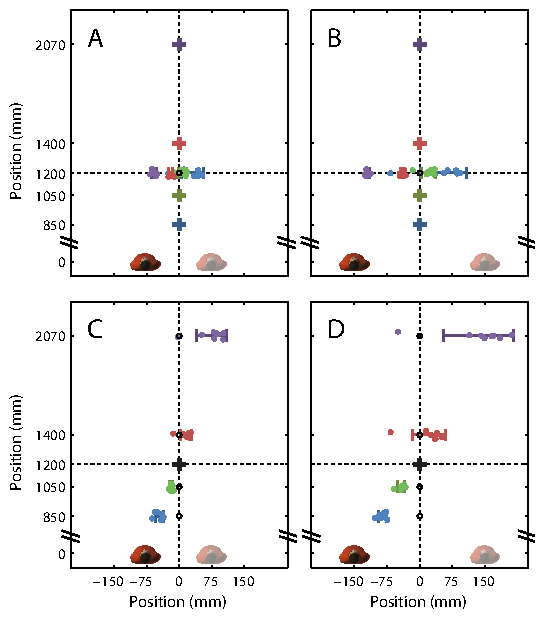
\includegraphics[width=0.75\textwidth]{src/paper2/figure3.pdf}
\end{figure}

To further analyze these observations, Figure 4 plots the bias values ({\textpm}SE across participants) as a function of gaze fixation FP (panel A), target location R (panel B) and reference location relative to gaze fixation FP - R (panel C). Both the location of FP and R, as well as the bias are expressed in units of degrees instead of millimeters because the former is more closely associated with native visual coordinates. (In practice, however, because of the large distance, visual angles are about proportional to the associated horizontal distances). While in panel A no clear relationship is observed ($R^2 = 0.09$, $F(1,14) = 1.32$; $p > 0.05$), panel B reveals only a weak linear relationship ($R^2 = 0.25$, $F(1,14) = 4.71$; $p < 0.05$). However, in panel C the data for all conditions are rearranged such that they fall into a single response curve. A linear fit shows a very strong correlation in this case ($R^2 = 0.97$, $F(1,14) = 483$, $p < 0.05$). This suggests that the observed errors almost solely depend on the location of R relative to gaze.

\begin{figure}
    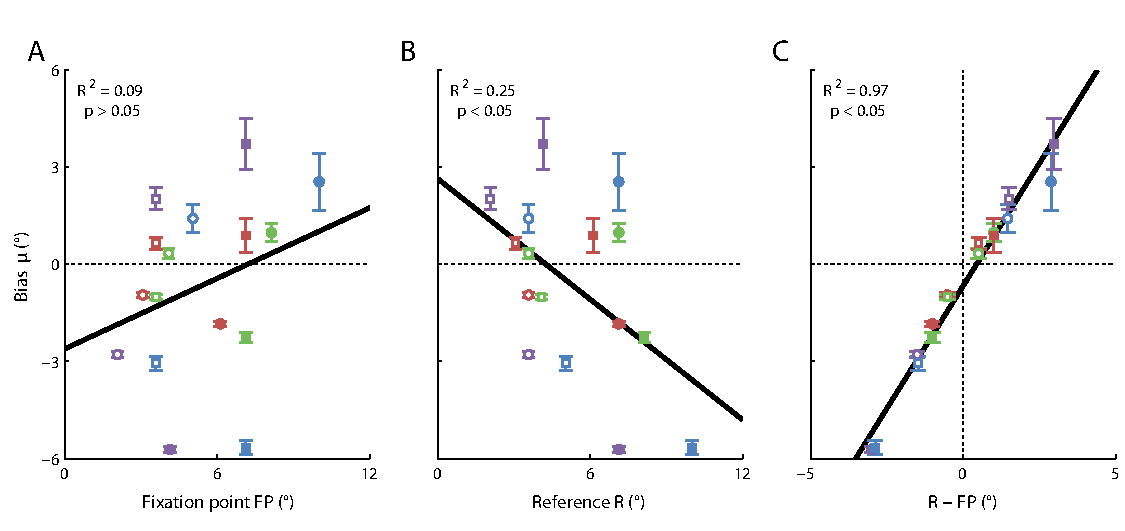
\includegraphics[width=1.0\textwidth]{src/paper2/figure4.pdf}
\end{figure}

To validate this notion, we fit two different models to explain the updating biases: a head- and gaze-centered model (see Eqs. 2 and 6 respectively, in Methods). Because the updating bias systematically depends on gaze, we expect the gaze-centered model to outperform the head-centered model. Indeed, the RMSE of the gaze-centered model was significantly lower (t-test; $t(7) = -3.68$, $p < 0.05$) than that of the head-centered model. Table 2 presents the RMSE values for both models and the fit-results of the gaze-centered model for each participant. According to this latter model, the best-fit value of the gain $\gamma$ (mean 0.25 \textpm0.08 SE) is considerably lower than the ideal value of one. In the Discussion we will address the possible implications of this small value.

% Table 2

Finally, in addition to accuracy, we also quantified the precision of the updated R. Figure 5 shows the standard deviation ($\sigma$ {\textpm}SE across participants) of the psychometric functions as a function of either FP (panel A), the head-centered location of R (panel B) or the gaze-centered location of R (panel C), in the same format as Fig. 4. No significant effects can be observed in panels A and B ($R^2 = 0.18$, $F(1,14) = 3.14$, $p > 0.05$ and $R^2 = 0.00$, $F(1,14) = 0.03$, $p > 0.05$ respectively). Panel C shows a significant linear relationship ($R^2 = 0.41$, $F(1,14) = 9.68$, $p < 0.05$). From this, we conclude that precision decreases for targets that are further or nearer in depth relative to fixation, and therefore also more peripheral in gaze-coordinates.

\begin{figure}
    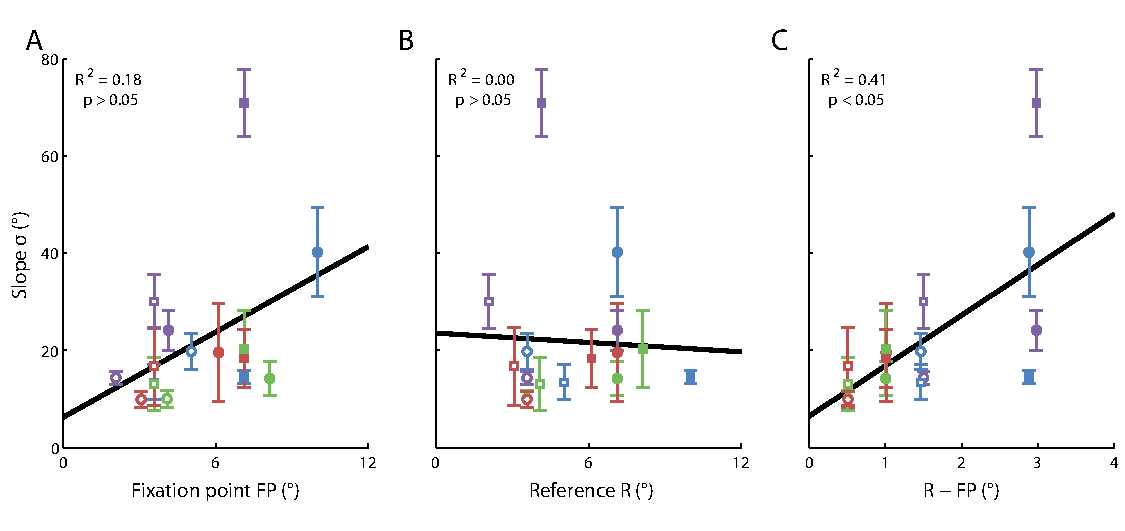
\includegraphics[width=1.0\textwidth]{src/paper2/figure5.pdf}
\end{figure}

\section{Discussion}

We investigated how the brain integrates retinal and extraretinal signals in order to maintain visual stability across combined eye and body motion. Participants had to remember the location of a world-fixed reference target, flashed in the periphery, while their body was passively translated and their binocular gaze actively changed in order to fixate a world-stationary target LED. When body motion reversed direction, a probe target was presented and the participant indicated whether it was shown to the left or right of the memorized reference. The resulting psychometric curves revealed substantial biases in the updating of the reference target, which increased with depth from fixation and reversed in sign for reference targets presented at opposite depths from fixation. In addition, precision of visual stability decreased when the distance between this target and the fixation point increased, likely due to the lower spatial resolution in the retinal periphery \cite{westheimer1982}. Geometric modeling suggests that these observations are consistent with spatial updating in a gaze-centered reference frame. In the following, we compare our results to previous work, and explore possible explanations of our observations in context of the gaze-dependent updating model.

\subsection{Relation to previous studies}

To our knowledge, there have been no other studies that have psychophysically investigated perceptual stability during combined eye and body motion. So far, related studies have tested spatial stability using paradigms in which participants make saccades or reaches to previously flashed targets after intervening self-motion (see Klier and Angelaki, 2008; Medendorp, 2011 for review). 
For actively generated self-motion, Medendorp et al. (2003b) had participants make saccade-vergence movements to remembered targets that were presented before they made a sidestep. Although their participants initially misperceived the targets, i.e. they underestimated the depths of distant targets and overestimated depths of near targets \cite{gogel1977, komoda1974, philbeck1997}, they accurately compensated for the intervening motion in the updating of the perceived target location, following the required non-linear updating patterns. Similar observations were made in relation to the updating of spatial locations across active self-motion for reaching \cite{admiraal2004, flanders1999, medendorp1999, vanpelt2007}. Compared to the present study, compensation for active intervening whole body motion was substantially better in all these studies.
Regarding passively induced self-motion, previous work by Isra\"el and Berthoz \nocite{israel1989} and more recent observations by Klier, Hess and Angelaki (2008) showed that human participants can also update the locations of saccade targets for passive whole body motion. Similar experiments in non-human primates have also demonstrated compensation for translational motion in the updating of saccadic space \cite{li2005a}. Although the amount of compensation depended on the depth of fixation, it was typically less than geometrically required (see their figure 4B), as in the present results. The same experiments were also conducted in labyrinthectomized monkeys, showing that their updating is even more compromised \cite{li2005b, wei2006}. This suggests that otolith information interacts with visual information to update saccade goals. 
Thus, in view of previous studies, our results are consistent with the notion that spatial ability is better maintained across active compared to passive body motion, perhaps due to the presence of efference copies of motor commands during active motion. Furthermore, based on the present findings it seems that perceptual updating is worse when compared to the action-oriented updating in previous studies. Should this be interpreted in favor of the proposal that visuospatial updating is organized in distinct processing pathways, one for conscious perception and one for the control of action \cite{goodale1992}? We do not want to suggest this. There may be other factors that contribute to the relatively low updating performance in the present study. Using geometric models (i.e., Eqs. 2 and 6) we will now explore such factors in more detail.

\subsection{Modeling implications}

In order to systematically explore possible explanations for the updating performance found in the present study, we now return to the head- and gaze-centered models of the updating mechanism presented in Eqs. 2 and 6 respectively. These models were inspired by the models proposed by Van Pelt and Medendorp (2007), with the addition of the possibility of a foveal bias. In the head-centered model (Eq. 2), the updating bias is proportional to the translation amplitude, but independent of reference and/or fixation point positions. However, since our data show a clear and systematic dependence on these positions (see Figs. 2-4), this model is not viable.
This leaves us with the gaze-centered model of Eq. 6, which incorporates these dependencies. Estimating the overall gain parameter ? in this gaze-centered model yielded a mean value of ? = 0.25 across participants. Since this ? is the product of parameters ? and ? (see Eq. 5), this entails that at least one of these parameters must be considerably smaller than one, the veridical value. That is, in the updating process the translation is perceived with a small gain (? << 1) and/or there is a distinct bias towards fixation depth (? << 1). We now explore the plausibility of these explanations in turn. 
For the perception of body translation at least two signals may be important: the vestibular signal from the otoliths and the changes in eye position while tracking the visual FP. Both linear acceleration (peak: 231 cm/s2) and frequency (0.63 Hz) were well above the detection thresholds of the otoliths \cite{benson1986, yu2012}. Furthermore, the firing rate of otolith afferents increases monotonically with acceleration in our frequency range \cite{fernandez1976, yu2012}, and can therefore be used to correctly decode acceleration. However, this does not mean that further processing of acceleration into a velocity or displacement signal is veridical \cite{merfeld2005}. In fact, it has been shown that the translational vestibuloocular reflex is not perfectly compensatory at the frequency that we have tested. However, when the vestibular signal is complemented by visual following mechanisms, participants are able to maintain fixation \cite{medendorp2002, paige1998}. This indicates that a near veridical percept of translation is possible by combining vestibular and eye position information. Yet, higher level processing of the translation signal might still be biased. For instance, the conversion of translated distance into an updating angle might be faulty, and/or the actual updating process itself could misinterpret an otherwise veridical updating angle. It has been shown that near-veridical updating takes place for e.g. reach targets \cite{henriques1998, vanpelt2007} where errors are attributed to the reference frame transformation instead. This suggests that the gaze-centered remapping process itself, which is thought to drive spatial updating, is not biased.
Thus, when considering previous work, it is most likely the higher level processing of the translation signal that governs the observed biases. One such processing step concerns the problem of attributing visual motion to either self-motion or object-motion \cite{vonhelmholtz1867}. If this attribution is flawed, it can have a profound influence on updating and might be the cause of our low updating gain. Support for this idea is found in work by Dyde and Harris (2008) who showed that participants make such attribution errors, in particular in conditions of passive translation and darkness, both of which apply to our study. In the active translation studies mentioned earlier, this effect is likely diminished by the presence of an efference copy that helps in disambiguating self-motion from object-motion.
A further explanation for our low overall gain is that depth perception of the reference point is biased (? << 1). Because the reference and probe lights were flashed for only 50ms at the zero velocity points of the sinusoidal motion and the head is unable to move relative to the body, depth perception of these lights is likely to be compromised. Actually, the spatial updating process that takes place in our experiment can alternatively be described in terms of a Bayesian model. To represent the brain's assumption that, lacking any precision information, the depth of peripheral stimuli is at or close to fixation point depth, such a model will involve a prior distribution centered at this fixation depth. The full specification of such a Bayesian model is beyond the scope of this paper. Here, we have opted for a more straightforward geometrical modeling approach (Eqs. 2 to 6), in which such a foveal depth bias appears in Eq. 4 with the weight 1 - ?. While such foveal influences have been reported previously \cite{brenner2008, mateeff1983}, for this to be the sole explanation for our low gain would require the foveal bias to be 80\%, which is quite extreme.
In conclusion, we have shown systematic biases in visual stability across combined eye and body movements. These biases are consistent with a gaze-centered updating model, with simple gain factors on both translation and depth perception.  

